\documentclass[12pt]{report}

\def\magyarOptions{defaults=hu-min}
\usepackage[magyar]{babel}
\usepackage[utf8]{inputenc}
\usepackage{t1enc}

\usepackage{times}

\usepackage{amsmath}
\usepackage{amssymb}
\usepackage{amsthm}

\usepackage{enumitem}
\usepackage{fancyhdr}
\usepackage{hyperref}
\usepackage{graphicx}
\usepackage{xcolor}

% Margins
\hoffset -1in
\voffset -1in
\oddsidemargin 35mm
\textwidth 150mm
\topmargin 15mm
\headheight 10mm
\headsep 5mm
\textheight 237mm

% URL style
\hypersetup{
    colorlinks=false, % Disable colorlinks for not coloring table of contents
}

\let\orighref\href
\renewcommand{\href}[2]{%
    \orighref{#1}{\textcolor{blue}{#2}}
}

\let\origurl\url
\renewcommand{\url}[1]{%
    \textcolor{blue}{\underline{\origurl{#1}}}
}

\newcommand{\todo}[1]{%
    \textcolor{red}{\textbf{TODO}}\footnote{\textcolor{red}{\textbf{TODO:} #1}}
}

\newcommand{\fixme}[1]{%
    \textcolor{red}{\textbf{FIXME}}\footnote{\textcolor{red}{\textbf{FIXME:} #1}}
}

\newcommand{\newpar}{\par\noindent\parskip=8pt}

\setdescription{
    style=standard,
    align=right,
    itemindent=2cm,
    labelwidth=2cm,
    leftmargin=2cm,
    %font=\sffamily\bfseries,
}

\def\title{A QtWebEngine modul fejlesztése}

\begin{document}

% EMPTY PAGE STYLE
\fancypagestyle{plain}{
    \fancyhf{}
    \fancyfoot[R]{\thepage}
    \renewcommand{\headrulewidth}{0pt}
}

% FOOTER & HEADER
\pagestyle{fancy}
\fancyhf{}
\fancyhead[L]{\title}
\fancyfoot[R]{\thepage}
%\fancyfoot[C]{\thepage}

%%% TITLE PAGE %%%
\thispagestyle{empty}
\begin{center}
    \vspace*{1cm}
    {\Large\textbf{Szegedi Tudományegyetem}}

    \vspace{0.5cm}
    {\Large\textbf{Informatikai Tanszékcsoport}}

    \vspace{3.8cm}
    {\LARGE\textbf{\title}}

    \vspace{3.6cm}
    {\Large Diplomamunka}

    \vspace{4cm}
    \begin{large}
        \begin{tabular}{c@{\hspace{4cm}}c}
            \emph{Készítette:}      & \emph{Témavezető:}        \\
            \textbf{Varga Péter}    & \textbf{Dr. Kiss Ákos}    \\
            programtervező          & egyetemi adjunktus        \\
            informatikus szakos     &                           \\
            hallgató                &
        \end{tabular}
    \end{large}

    \vspace*{2.3cm}
    \begin{Large}
        Szeged

        \vspace{2mm}
        2016
    \end{Large}
\end{center}


%%% TABLE OF CONTENTS %%%
\tableofcontents

%%% PROLOGUE %%%

\chapter*{Feladatkiírás}
\addcontentsline{toc}{section}{Feladatkiírás}

\noindent
A \texttt{QtWebEngine} modul bővítése úgy, hogy a \texttt{QtWebKit} modult használó
fejlesztők könnyen portolhassák a projektjüket \texttt{QtWebEngine}-re. Az újonnan
implementált funkciókat tesztelni kell.

\bigskip
\noindent
A tesztelésre lehetőséget nyújt a \texttt{Qt auto test}
keretrendszere, viszont bizonyos funkciók nem tesztelhetőek megfelelően \texttt{auto}
tesztekkel, továbbá nem biztosítható teljes lefedettség. A probléma kiküszöbölésére
példa alkalmazás(ok) implementálására van szükség, amelyet a fejlesztő használhat
``manuális'' tesztelésre, hibakeresésre, továbbá a forráskódja funkciók dokumentálására is
felhasználható.

\bigskip
\noindent
A fejlesztés során az alábbi szempontokat kell figyelembe venni:
\begin{itemize}
    \item[\texttt{o}] Bináris kompatibilitás megtartása korábbi \texttt{QtWebEngine}
        verziókkal: publikus API-ban a változtatások számát minimalizálni kell,
        meglévő API-t (függvény, \\
        property, signal, stb.) módosítani vagy eltávolítani
        nem lehet.
    \item[\texttt{o}] Törekvés kompatibilitásra a \texttt{QtWebKit}-el.
        A \texttt{QtWebEngine}-hez adott új \mbox{API-k} ne térjenek el
        (névben, paraméterezésben, stb.) az eredeti \texttt{QtWebKit} API-tól, hacsak ezt
        \dots \todo{milyen esetekben volt erre szükség?}
        nem indokolja.
    \item[\texttt{o}] Törekedni kell arra, hogy a Quick és Widget API hasonlítson egymásra,
        amennyire csak lehet.
    \item[\texttt{o}] Az új funkcionalitásokhoz \texttt{auto} tesztet kell készíteni,
        ahol ez megoldható.
    \item[\texttt{o}] Qt 5.6-tól minden új funkcionalitást dokumentálni kell.
\end{itemize}


\chapter*{Tartalmi összefoglaló}
\addcontentsline{toc}{section}{Tartalmi összefoglaló}
\begin{itemize}
    \item[\texttt{o}] \textbf{A téma megnevezése:} \\
        A \texttt{QtWebEngine} modul \dots
        \todo{Találjunk jobb címet a dolgozatnak. A cím nem utal arra, hogy a QtWebEngine
        alkalmazásáról is szól egy egész fejezet.}
    \item[\texttt{o}] \textbf{A megadott feladat megfogalmazása:} \\
        A \texttt{QtWebEngine} modul bővítése olyan funkciókkal (feature-ök),
        amelyekkel az előd (\texttt{QtWebKit}) már rendelkezett. A cél, hogy a
        \texttt{QtWebKit} felhasználók átállását megkönnyítsük és, hogy egyáltalán
        lehetővé tegyük.
        \todo{Hasonló probléma, mint a címnél. A feladatkiírás nem szól a QtWebEngine
        alkalmazását bemutató fejezetről.}
    \item[\texttt{o}] \textbf{A megoldási mód:} \\
        Részvétel a \texttt{QtWebEngine} project fejlesztésében. Az új funkciók
        megvalósítása \texttt{C++} nyelven.
    \item[\texttt{o}] \textbf{Alkalmazott eszközök, módszerek:} \\
        A fejlesztés \texttt{GNU/Linux} rendszeren, \texttt{QtCreator} fejlesztői
        környezetben (IDE) történt. A hibakereséshez \texttt{GDB}-t használtam.
        \texttt{Makefile}-ok legenerálását a project file-okból a \texttt{qmake} végzi.
        A project fordítása \texttt{Linux}-on a \texttt{GNU Toolchain}-el (\texttt{GCC 5.3}),
        \texttt{Os X}-en \texttt{Xcode} -al (\texttt{Xcode 7.2.1}), \texttt{Windows}-on pedig
        \texttt{MSVC 2013} 32-bites verziójával történt. A verzió-követéshez \texttt{Git}-et
        használtam. A teszteléshez szükséges keretrendszert és a teszteket a \texttt{Qt}
        repository-k tartalmazzák.
    \item[\texttt{o}] \textbf{Elért eredmények:} \\
        A munka megkezdése óta minden \texttt{QtWebEngine} verzióhoz sikerült olyan funkciót
        hozzáadni vagy kijavítani, amely a \texttt{QtWebKit} API-ban elérhető:
        \todo{Ide jöhet a lista a verziókról és feature-ökről}, 5.6: Authentication Dialog,
        5.7: Favicon Manager \todo{A felsorolás lehetne hivatkozás az alfejezetekre}
    \item[\texttt{o}] \textbf{Kulcsszavak:} \\
        \texttt{QtWebEngine}, \texttt{QtWebKit}, \texttt{Qt}, \texttt{Chromium}, \\
        \texttt{Chromium Content API}, \texttt{Web}, \texttt{HTML5}, \texttt{C++}, \\
        \texttt{Quick}, \texttt{QML}, \texttt{Widget}, \texttt{WebEngineView} \\
        \todo{Lista bővítése és formázása}
\end{itemize}

%%% CONTENT %%%

\chapter*{Bevezetés}
\addcontentsline{toc}{section}{Bevezetés}
\begin{itemize}
    \item Mi a cél?
    \item Bemutatom a \texttt{Chromium}-ot, a \texttt{Qt}-t és a kettőjük kapcsolatát
    \item Bemutatom, hogy a QtWebEngine fejlesztéséhez milyen funkcionalitásokkal járultam
        hozzá
    \item 1-2 mondat: volt más fejlesztés is: karbantartás, tesztek, bug fix
    \item Miért jó ez? Nem gyors, viszont cross-platform, és könnyű ``látványos'' dolgokat
        készíteni
    \item Könnyű böngészőt készíteni.
        \begin{itemize}
            \item Proof: utolsó fejezet, a példaböngészőről
        \end{itemize}
\end{itemize}

\chapter{Áttekintés: \mbox{Chromium + Qt = QtWebEngine}}

\section{Chromium}
A \texttt{Chromium} a Google által fejlesztett, nyílt forrású web böngésző projekt. Nagy
része \texttt{C++} nyelven íródott. Támogatja napjaink legnépszerűbb operációs rendszereit
(``Cross-Platform''), legyen az desktop (Windows, Linux, OS X) vagy mobil (Android, iOS,
QNX).
A \texttt{Chromium} nem egy böngésző alkalmazás, hanem egy tabokat használó ablakkezelő
vagy shell a web-hez.

\subsection{Chrome}
A Google saját \texttt{Chromium}-ra épülő böngésző alkalmazása a \texttt{Google Chrome}.
Ez az alkalmazás \texttt{Chromium}-mal szemben nem nyílt forrású, viszont a böngésző
megvalósításának nagy része a \texttt{Chromium} projektben megtalálható.
A \texttt{Chrome} nem nyílt részei például a beépített \texttt{Adobe Flash Player}
(\texttt{Pepper Flash Player}) és az automatikus frissítésekért felelős modul
(\texttt{GoogleUpdate}). Egy másik, népszerű \texttt{Chromium}-ra épülő böngésző alkalmazás
az \texttt{Opera}.

\subsection{Blink}
\newpar
A \texttt{Chromium} 27-es verziójától kezdve a \texttt{Blink} böngésző motort használja.
A böngésző motor elsődleges feladata a webes tartalom megjelenítése a képernyőn. Talán
ebből is látszik, hogy a \texttt{Blink} talán a legfontosabb komponense
a \texttt{Chromium}-nak. A \texttt{Chromium} a 27-es verzió előtt \texttt{WebKit}-et
használt, a Google ezt a projektet forkolta és nevezte el \texttt{Blink}-nek. Pontosabban,
a \texttt{Blink} nem a teljes \texttt{WebKit} forkja, hanem csak annak egy részének, a
\texttt{WebCore}-nak.

\newpar
A \texttt{Blink} nem tartalmazza a \texttt{WebKit}-ben alkalmazott multi-process
architektúrát és sandboxing-ot, ezek a feladatok a \texttt{Chromium} más szintjein jelennek
meg így egyszerűbbé téve a \texttt{Blink} implementációját. Továbbá, a \texttt{WebKit} része
a \texttt{JavaScriptCore} JavaScript motor is, ami a \texttt{Blink}-be már nem került bele,
hiszen a \texttt{Chromium}-nak van sajátja, a \texttt{V8}.
Ettől eltekintve a \texttt{Blink} még mindig nagyon hasonlít a
\texttt{WebCore}-ra/\texttt{WebKit}-re, a \texttt{Chromium}
forrásában és könyvtár struktúrájában még mindig \texttt{WebKit} néven hivatkoznak erre a
komponensre. Például, a \texttt{Blink} forrása a \\
\texttt{third\_party/WebKit} könyvtárban van.

\newpar
Már említettem, hogy a \texttt{Blink}, mint böngésző motor felel a webes tartalmak
megjelenítésért. Ennek működése fontos a \texttt{QtWebEngine} szempontjából, ezert ezt itt
röviden részletezném.
A \texttt{Blink} a web oldal tartalmát feldolgozza (parse-olja), és a HTML elemekből
\texttt{Node} objektumokat gyárt. Ezeket a \texttt{Node}-okat egy fába rendezi, amit
\texttt{DOM} (Document Object Model) fának hívnak. A fának a gyökér \texttt{Node}-ja mindig,
az úgynevezett, \texttt{Document Node}. A \texttt{DOM} fa építése során, a motor, minden
megjeleníthető \texttt{Node}-hoz egy \texttt{RenderObject}-et rendel. A \texttt{DOM} fa
építésével párhuzamosan egy másik fát is épít a \texttt{RenderObject}-ekből, a
\texttt{Render Tree}-t. A \texttt{RenderObject} ``tudja'', hogyan kell a \texttt{Node}-ot
megjeleníteni. Továbbá, bizonyos \texttt{RenderObject}-hez \texttt{RenderLayer}-t is
rendel, amiből egy újabb fát épít: \texttt{RenderLayer Tree}.
\todo{Mi a forrás hivatkozásának hivatalos formája? Lábjegyzetbe? Bibliográfiából? Mindkettő?}

\begin{figure}[h]
    \centering
    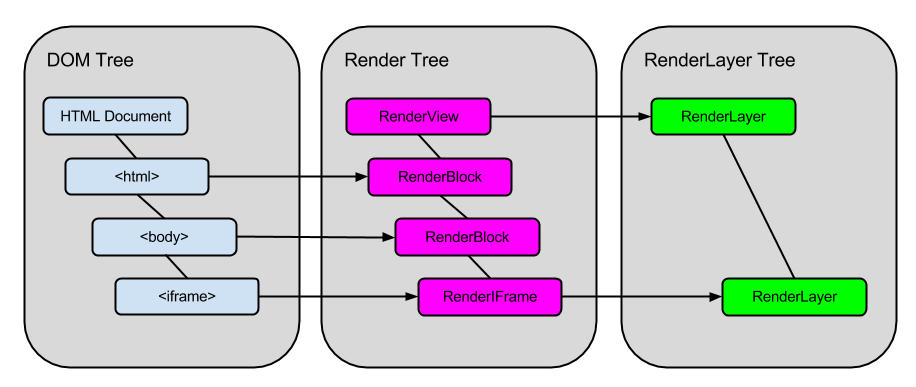
\includegraphics[scale=0.45]{rendering_trees}
    \caption{
        \label{figure-rendering-trees}
        Rendering Trees (forrás: \url{https://www.chromium.org})
        %https://www.chromium.org/developers/design-documents/oop-iframes/oop-iframes-rendering
    }
\end{figure}

\newpar
Ahogy az \ref{figure-rendering-trees} ábrán is látszik a \texttt{DOM Tree} és a
\texttt{Render Tree} szinte azonos, csak a \texttt{Render Tree} csak a megjeleníthető
\texttt{Node}-okat tartalmazza. Míg a \texttt{RenderLayer Tree} a \texttt{Render Tree} egy
lecsupaszított változata, amit a \texttt{renderer} fog használni a rajzoláshoz.
A \texttt{RenderLayer}-ből elérhetőek a \texttt{RenderObject}-ek (amik tudják, hogyan
kell kirajzolni a tartalmat), a \texttt{RenderLayer Tree} pedig hordozza azt az információt,
hogy milyen sorrendben kell rajzolni és, hogy milyen átfedések lehetnek.

\newpar
Az, hogy a rajzolás ezek után hogyan történik az függ attól, hogy van e elérhető hardveres
gyorsítás. Ha nincs, akkor szoftveres renderelés történik úgy, hogy a
\texttt{RenderLayer Tree}-n keresztül megfelelő sorrendben bejárják a
\texttt{RenderObject}-eket és kirajzoltatják őket egy közös bitmap-re. Ha kész, ez a bitmap
lesz elküldve a böngésző alkalmazásnak (pl. \texttt{Chrome}) megjelenítésre. Szoftveres
renderelés esetén a rajzolást a \texttt{Skia} grafikus motor végzi.

\newpar
Ha van elérhető hardveres gyorsítás, akkor az eljárás valamivel bonyolultabb. Az egésznek az
a lényege, hogy a \texttt{RenderObject} nem bitmap-be ``rajzolja bele magát'', hanem 3D API-n
keresztül (\texttt{OpenGL} vagy Windows-on \texttt{D3D}) utasításokat küld közvetlenül a
GPU-nak (grafikus processzor). Ezt az eljárást már a \texttt{Chrome Compositor} (\texttt{CC})
végzi.

\newpar
A \texttt{Chrome Compositor} már nem része a \texttt{Blink}-nek
(ennek az az oka, hogy most már a \texttt{Chromium} a browser UI megrajzolásához is a
\texttt{Chrome Compositor}-t használja).
Ahhoz, hogy a compositor ki tudja rajzolni a \texttt{DOM}-ban tárolt tartalmat,
további layer absztrakciókra van szükség:
\begin{center}
    \texttt{RenderLayers} $\rightarrow$ \texttt{GraphicsLayers} $\rightarrow$
    \texttt{WebLayers} $\rightarrow$ \texttt{CC Layers}
\end{center}

\newpar
A compositor a végeredményt nem bitmap-be, hanem textúrába ``rajzolja''. Az elkészült
textúrák a GPU memóriájában vannak tárolva és \texttt{texture mailbox} segítségével
azonosítják. A \texttt{texture mailbox} egy \texttt{OpenGL extension}, ami egyedi és globális
string azonosítót rendel a textúrához és lehetővé teszi, hogy más \texttt{OpenGL context}-en
is elérhető legyen a textúra, ami normális esetben nem lenne megosztva.

\newpar
A \texttt{texture mailbox}-nak hála az összeállított képet nem kell az \texttt{IPC}-n
(\texttt{Inter-Process Communication}) keresztül megosztani a process-ek között
(mint a szoftveres rendering esetében), hanem a GPU memórián keresztül bármelyik
process hozzáférhet a textúrához.

\subsection{Multi-Process Architektúra}
\newpar
\begin{itemize}
    \item Cél:
        \begin{itemize}
            \item Ne ``álljon'' a UI, mikor a browser dolgozik
            \item Hiba esetén ne szálljon el az egész browser
        \end{itemize}
    \item Process-ek:
        \begin{itemize}
            \item Browser Process (main process)
            \item Render Process (minden tabhoz)
            \item Plugin-oknak (NPAPI) saját process
            \item GPU process
        \end{itemize}
    \item GPU Process
        \begin{itemize}
            \item Mit is csinál -> compositing on GPU
            \item Security
            \item Direct 3D API calls (D3D, OpenGL)
            \item MailboxTexture?
            \item Model-ek:
                \begin{itemize}
                    \item Old Rendering Model
                    \item Hardware Accelerated Model
                \end{itemize}
        \end{itemize}
\end{itemize}

\subsection{Chromium Content Module}
\begin{itemize}
    \item WebKit-hez képest a különbség -> WebKit-től eltérő megközelítés
    \item Content API
    \item Unstable API
    \item Mit is jelent ez?
    \item Felépítés
    \item Design Pattern
        \begin{itemize}
            \item Delegate interfaces
            \item Observer interfaces
            \item Callbacks
        \end{itemize}
\end{itemize}

\subsection{Felépítés}
\newpar
\todo{Ábra ide}

\subsection{Verzió?}
\newpar
Jelenleg hanyas verzió? Esetleg pár szó a releasekről?


\section{Qt}
\begin{itemize}
    \item Mi ez?
        \subitem Cross-platform, open source, fejlesztő környezet, framework
        \subitem \texttt{C++} függvénykönyvtár
    \item Egy kis történelem:
        \subitem Trolltech -> Nokia -> Digia -> The Qt Company
    \item GUI fejlesztés. 2 fajta megközelítés:
        \begin{enumerate}
            \item Widget
            \item Quick
        \end{enumerate}
    \item Verziók, hol tartunk, honnan jöttünk?
    \item Moduláris felépítés
\end{itemize}

\subsection{Qt Web}
\begin{itemize}
    \item Az Allan féle előadásból mehet egy kis áttekintés
    \item QtWebKit
    \item QtWebView (natív WebView, Android)
    \item QWebChannel
    \item QtWebEngine
    \item etc.
\end{itemize}

\section{QtWebEngine}
\begin{itemize}
    \item Qt module
    \item Ez az unstable API felé húzott stable API
    \item ``Együttműködés'' (integrálhatóság) más Qt API-kal
    \item OpenGL nélkül nem megy
    \item SceneGraph
    \item Qt függőségek
        \begin{itemize}
            \item qtbase
            \item qtdeclarative
            \item \dots
        \end{itemize}
    \item Karbantartási munkák: rendszeres Chromium update
\end{itemize}

\subsection{QtWebEngine Process}
\begin{itemize}
    \item Hogyan indul?
    \item Miért felel?
        \begin{itemize}
            \item Rendering
            \item etc.
        \end{itemize}
    \item IPC kommunikáció a process-ek között
    \item Thread-ek
    \item Single Process mode
\end{itemize}

\subsection{QtWebEngine Core}
\begin{itemize}
    \item Mi van benne?
    \item Új (5.7): publikus API, mire jó?
    \item Design Pattern
        \begin{itemize}
            \item Delegate osztályok
            \item Adapterek
        \end{itemize}
    \item \dots
\end{itemize}

\subsection{QtWebEngine API}
\begin{itemize}
    \item D pointeres dolog (private class-ok)
    \item Bináris kompatibilitás
    \item Miért a 2 API?
    \begin{itemize}
        \item A Quick a fontosabb
        \item A 2 API között vannak funkcióbeli különbségek (``az egyik tudja, a másik nem'')
    \end{itemize}
\end{itemize}

\subsubsection{Widget}
\begin{itemize}
    \item Szinkron API -> könnyebb tesztelés
\end{itemize}

\subsubsection{Quick}
\begin{itemize}
    \item Aszinkron API -> állandó probléma a tesztelésnél
        \begin{itemize}
            \item Bizonyos események (signal-ok) bekövetkezésének a sorrendje nem garantált
        \end{itemize}
\end{itemize}

\section{Összegzés}
\begin{itemize}
    \item TODO: egy ábra jöhet a felépítésről
    \item Hogyan kapcsolódnak a részek egymáshoz?
\end{itemize}


\chapter{Új funkciók a QtWebEngine-ben}

\section{Navigation History}

\begin{itemize}
    \item Hiányzó Quick API megvalósítása
    \item Backward, Forward list model
    \item TODO: Example gyártása?
\end{itemize}
\pagebreak

\section{Find Text}
\begin{itemize}
    \item Csak Quick API
    \item Tesztek portolása QtWebKit-ből
\end{itemize}
\pagebreak

\section{Log Level}
\fixme{Ez nem hagyományos értelemben vett API és a \texttt{QtWebKit}-ben nem is volt ilyen.
Kell ez?}
\begin{itemize}
    \item Parancssori kapcsoló
    \item Hibakeresés
    \item \texttt{-{}-log-level}
\end{itemize}
\pagebreak

\section{Test Support API}
\fixme{Ez sem volt a \texttt{QtWebKit}-ben. Ez nagyon internal dolog, de fontos lépés a
tesztelés szempontjából, továbbá egy lépéssel közelebb kerültünk az \texttt{experimental}
API eltávolításához.}
\begin{itemize}
    \item Olyan feature-ök tesztelése ami nem jelenhet meg a publikus API-ban
    \item Pl. error page, az error page signal-okat elrejtjük a fejlesztő elől, de tesztelni
        kell.
    \item Előfordulhat, hogy a fejlesztő saját felelőségére használja
    \item Nincs dokumentálva
\end{itemize}
\pagebreak

\section{Form Validation}
\fixme{Ez sem volt a \texttt{QtWebKit}-ben, viszont fontos lépés a \texttt{HTML5} támogatás
felé. Talán a \texttt{HTML5}-öt is be kellene venni az ismertetőbe.}
\begin{itemize}
    \item kódnév: Bubi
    \item Message Bubble
    \item HTML5 feature
    \item Chromium callback megvalósítása
    \item Quick és Widget API-ban kétféleképpen megrajzolt buborék
    \item Test Support API teszt
\end{itemize}
\pagebreak

\section{Localization}
\todo{Hasonló a Log Level-hez. Ez tulajdonképpen nem API és Chromium specifikus.}
\begin{itemize}
    \item Tesztelés miatt: csak angol nyelvű hibaüzenetek
    \item Qt API-n keresztül beállított lokalizáció használata
    \item \texttt{-{}-lang} parancssori kapcsoló lokalizáció felüldefiniálására
\end{itemize}
\pagebreak

\section{Authentication Dialog}
\begin{itemize}
    \item Dialog Quick-hez: \texttt{AuthenticationDialogController}
    \item HTTP authentication
        \begin{itemize}
            \item Simple authentication
            \item Kerberos?
        \end{itemize}
    \item Proxy authentication
    \item Jelszóval védett oldalak esetén dobjon fel ablakot a felhasználó név és jelszó
        megadásához
        \begin{itemize}
            \item pl. \url{wiki.sed.hu}
        \end{itemize}
    \item Probléma, authentikált oldalak esetén nem lehet letölteni a favicon-t
        \begin{itemize}
            \item Widget: QNAM (QNetworkAccessManager) tölti le az ikont, viszont nem kapja
                meg a bejelentkezéshez szükséges credentials-t
            \item Quick: Image QML elem van használva a kép megjelenítésére (ikon támogatás a
                QML-ben nincs).
            \item Az Image QML elem implicit elvégzi a letöltést, ami a felhasználó elől
                rejtve marad => nincs lehetőség authentikációra
        \end{itemize}
    \item Empty credentials és cancel
\end{itemize}
\pagebreak

\section{Favicon Manager}
\begin{itemize}
    \item Ikonok letöltése a Chromium Content API-n keresztül
    \item Az összes ikon letöltése és a legjobb minőségű propagálása
        \begin{itemize}
            \item Az eredeti megvalósításban a touch ikonok nem voltak kezelve
            \item Fontos lehet érintő kijelzős eszközökön vagy akár desktop gépeken is
            \item A history vagy könyvjelzők megjelenítés nagy méretű ikonokkal
        \end{itemize}
    \item Konfigurálhatóság a WebEngineSettings-en keresztül (``Icon Download Modes'')
        \begin{itemize}
            \item Letilthatóak lehessenek az ikonok (sávszélesség, sebesség, saját icon
                manager)
            \item Desktop-on alapból nincsenek bekapcsolva a touch ikonok, de engedélyezni
                lehessen őket
        \end{itemize}
    \item Terv: egy QIcon-ban ``összegyúrva'' az összes ikon
        \begin{itemize}
            \item a felhasználó extra API nélkül könnyedén kiválaszthatja a számára
                megfelelő méretet
            \item Quick esetében az Image átméretezésekor a megfelelő felbontású ikon
                kerül betöltésre
        \end{itemize}
    \item widget API-ra példa QtWebKit-ből
        \begin{itemize}
            \item Azért van szükség módosításra
            \item kész dokumentáció
        \end{itemize}
    \item Quick API-hoz icon image provider
        \begin{itemize}
            \item problémák: hogyan kössük be a manager-t? Hol kössük be a provider-t az
                engine-be?
        \end{itemize}
    \item Hosszabb távú tervek (Qt 5.8)
        \begin{itemize}
            \item API bővítése az elérhető ikonok listázására és explicit letöltésére
            \item Icon database: merevlemezen tárolt ikonok (oldal betöltése előtt is
                elérhető legyen vagy offline módban)
        \end{itemize}
\end{itemize}
\pagebreak


\chapter{Egy példa browser megvalósítása}
\textbf{Szempontok:}
\begin{itemize}
    \item Screenshot-ok legyenek a browser-ről
    \item Csak a lényeget részletezni (funkciók megjelenése), a ``körítés'', design-t csak
        megemlíteni
    \item QML példakód a funkciókra
\end{itemize}

\noindent
\textbf{Gondolatok:}
\begin{itemize}
    \item Gyors billentyűre felugró pop-up, amibe az URL-t lehet írni. Animált (halványodik),
        félig áttetsző
    \item Az URL pop-up-nak legyen saját history-ja a memóriában (csak addig él amíg a
        program fut). Indításkor a navigation history-ból legyen inicializálva.
        Automatikus URL kiegészítés.
    \item Legyenek az oldalakról screenshot-ok tárolva. Az URL pop-up a felajánlott oldalakkal
        együtt mutatja a screenshot-ot.
    \item A tabok bal oldali sávon legyenek, vertikális listában. Indok: desktop browser,
        a monitorok szélesek
    \item A tab bar-hoz nem használható a Quick TabView
    \item Tab bar-nak 3 állapota megjelenés szerint:
        \begin{description}
            \item[hidden] Rejtett mód
            \item[compact] ``Keskeny'' mód. Csak ikon, vagy ikon és alatta a title.
            \item[full] A tab teljes szélességében
        \end{description}
    \item Módok között a váltás animált
    \item Jobb oldalt Bookmark Bar hasonló módokkal mint a Tab Bar
    \item A Bookmark Bar-on a legfelső ikon/bejegyzés a menü
    \item Menü dialog-ok animálva jelennek meg, amely mögött a \texttt{WebEngineView}
        megváltozik. Például, összemegy, elhalványul, mindkettő, stb.
    \item Tab váltáskor az aktuális WebEngineView animálva kiúszik a képernyőről és az
        új beúszik (slide?)
    \item A tabok rendezhetőek lehessenek a Tab bar-on.
    \item A tabok csoportokba rendezhetőek legyenek.
    \item A tab felett pár másodpercig tartott egérkurzor preview-t jelenít meg a \\
        \texttt{WebEngineView}-ról
    \item Egyedi dialog ablakok, ha addig elkészül a custom UI delegate
\end{itemize}

\noindent
\textbf{Funkciók megjelenése a példa browserben:}
\begin{description}
    \item[Navigation History] Legyen külön ``navigator'' ablak. Listában lépkedek az
        elemeken, kicsinyített nézetben látszik az oldal (esetleg screenshot?). Klikk-re
        kilép a navigátorból és megnyitja az oldalt.
    \item[Find Text] Ctrl+f shortcut -> animált pop-up. Regexet be lehetne-e adni?
    \item[Log Level] Példa browser indításakor \texttt{-{}-log-level} kapcsolóval
    \item[Test Support API] --
    \item[Form Validation] Screenshot a buborékról
    \item[Localization] Példa browser indításakor \texttt{-{}-lang} kapcsolóval
    \item[Authentication Dialog] Felül definiálni Custom UI delegate-el ha meg lesz
    \item[Favicon Manager] Nagy méretű ikonok: tab, bookmark (kompakt mód), URL pop-up
\end{description}

\addtocontents{toc}{\ }
\chapter*{Összefoglaló}
\addcontentsline{toc}{section}{Összefoglaló}
\begin{itemize}
    \item Eredmények és összegzés
    \item \todo{Van erre szükség? Mit lehet ebbe beleírni?}
\end{itemize}


%%% EPILOGUE %%%

\begin{thebibliography}{9}
    \addcontentsline{toc}{section}{Irodalomjegyzék}

    \bibitem{Google}
        Content API overview, \url{http://valami}

    \bibitem{Kai Koehne}
        QtWebEngine, taming? the beast, \url{http://www.youtube.com/...}
\end{thebibliography}


\chapter*{Nyilatkozat}
\addcontentsline{toc}{section}{Nyilatkozat}

\noindent
Alulírott Varga Péter programtervező informatikus MSc szakos hallgató, kijelentem, hogy a
dolgozatomat a Szegedi Tudományegyetem, Informatikai Tanszékcsoport Szoftverfejlesztés
Tanszékén készítettem, programtervező informatikus MSc diploma megszerzése érdekében.

Kijelentem, hogy a dolgozatot más szakon korábban nem védtem meg, saját munkám eredménye
és csak hivatkozott forrásokat (szakirodalom eszközök, stb.) használtam fel.

Tudomásul veszem, hogy a diplomamunkámat a Szegedi Tudományegyetem Informatikai Tanszékcsoport
könyvtárában, a helyben olvasható könyvek között helyezik el.

\vspace*{2cm}

\begin{tabular}{lc}
    Szeged, \today \hspace{2cm} & \makebox[6cm]{\dotfill} \\
                                & aláírás
\end{tabular}


\chapter*{Köszönetnyílvánítás}
\addcontentsline{toc}{section}{Köszönetnyílvánítás}

\noindent
Szeretnék köszönetet mondani Dr. Kiss Ákos témavezetőmnek a téma kutatása alatt nyújtott
támogatásáért és a diplomamunkám megírásában nyújtott segítségéért.

Ezen kívül szeretnék köszönetet mondani a \textit{The Qt Company} és a
\textit{Szegedi Tudományegyetem Szoftverfejlesztés Tanszék} volt es jelenleg is a QtWebEngine
projekten dolgozó munkatársainak a beszélgetésekért és a közösségnek benyújtott munkám
ellenőrzéséért és befogadásáért.


\chapter*{Mellékletek}
\addcontentsline{toc}{section}{Mellékletek}

\noindent
DVD lemez mely tartalmazza:
\begin{itemize}
    \item \texttt{QtWebEngine} modul \texttt{Git} repository-ját
    \item A bemutatott funkciókat megvalósító patch-eket
    \item A példa böngésző forráskódját
\end{itemize}

\end{document}
